147. \begin{figure}[ht!]
\center{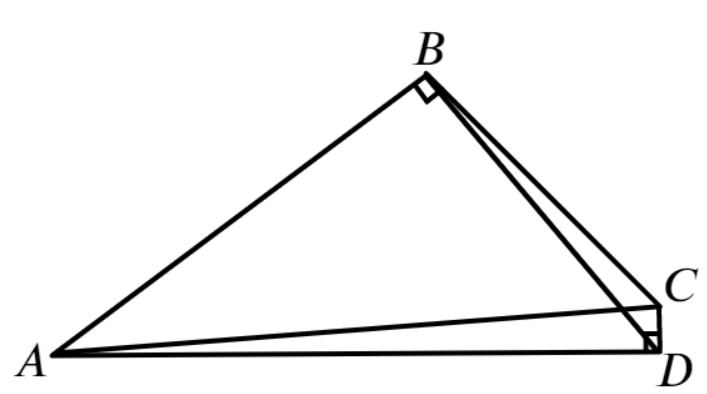
\includegraphics[scale=0.35]{g9-147.png}}
\end{figure}\\
Найдём $\angle C=360^\circ-90^\circ-90^\circ-45^\circ=135^\circ.$ Тогда по теореме косинусов $BD^2=16+18-2\cdot4\cdot3\sqrt{2}\cdot\left(-\cfrac{\sqrt{2}}{2}
ight)=58,\ BD=\sqrt{58}$ и $18=16+58-2\cdot4\cdot\sqrt{58}\cos(\angle DBC),\ \cos(\angle DBC)=\cfrac{7}{\sqrt{58}}.$ Так как $\angle B+\angle D=180^\circ,$ четырёхугольник $ABCD$ является вписанным и $\angle DBC=\angle DAC.$ Найдём $\sin(\angle DAC)=\sqrt{1-\cfrac{49}{58}}=\cfrac{3}{\sqrt{58}}=\cfrac{CD}{AC}=\cfrac{3\sqrt{2}}{AC},$ откуда $AC=2\sqrt{29}.$
ewpage
oindent
